\documentclass[11pt,a4paper,UTF8,fontset=fandol]{ctexart}

\usepackage[a4paper,margin=2.45cm,headheight=14pt]{geometry}
\usepackage{booktabs}
\usepackage{tabularx}
\usepackage{array}
\usepackage{longtable}
\usepackage{float}
\usepackage{enumitem}
\usepackage{setspace}
\usepackage{fancyhdr}
\usepackage[hidelinks]{hyperref}
\usepackage{microtype}
\usepackage{graphicx}
\usepackage{xcolor}
\usepackage{tikz}
\usetikzlibrary{arrows.meta,positioning,calc}

\hypersetup{
  pdftitle={语音驱动 PowerPoint 编辑 Agent：SURF 项目实验报告},
  pdfauthor={},
  pdfsubject={从 PPTArena 复现到 ASR + Agent 实验},
  pdfkeywords={SURF, PowerPoint, PPTArena, PPTPilot, ASR, Agent}
}

\setstretch{1.25}
\setlength{\parindent}{2em}
\setlength{\parskip}{0pt}
\setlength{\tabcolsep}{5pt}
\renewcommand{\arraystretch}{1.25}
\setlist[itemize]{leftmargin=2em,itemsep=2pt,topsep=3pt}
\setlist[enumerate]{leftmargin=2.4em,itemsep=2pt,topsep=3pt}

\ctexset{
  section={
    format=\zihao{3}\bfseries,
    beforeskip=1.2em,
    afterskip=0.55em
  },
  subsection={
    format=\zihao{4}\bfseries,
    beforeskip=0.9em,
    afterskip=0.35em
  }
}

\pagestyle{fancy}
\fancyhf{}
\fancyhead[L]{\small SURF 项目实验报告}
\fancyhead[R]{\small Voice-to-PPT Agent}
\fancyfoot[C]{\small \thepage}
\renewcommand{\headrulewidth}{0.4pt}
\renewcommand{\footrulewidth}{0pt}

\newcolumntype{Y}{>{\raggedright\arraybackslash}X}
\newcolumntype{C}[1]{>{\centering\arraybackslash}p{#1}}
\newcolumntype{L}[1]{>{\raggedright\arraybackslash}p{#1}}

\newcommand{\result}[1]{\textbf{#1}}
\newcommand{\pp}{个百分点}

\begin{document}

\begin{center}
\vspace*{1.8cm}
{\zihao{1}\bfseries 语音驱动 PowerPoint 编辑 Agent\par}
\vspace{0.8em}
{\zihao{3}\bfseries SURF 项目实验报告\par}
\vspace{1.2em}
{\large 2026 年 7 月\par}
\end{center}
\thispagestyle{empty}

\vspace{1.6em}
\begin{abstract}
本项目以 PPTArena 论文提出的 PPTPilot 为执行 Agent，面向 SURF 项目“语音指令到可执行幻灯片编辑”的研究目标，完成了论文代码本地化、GUI 复现、CLI 重构、双 ASR 接入和端到端实验。最终系统能够保存音频转写、Agent 运行日志、编辑后 PPTX 及核验结果。

实验选用 faster-whisper large-v3-turbo 和 Qwen3-ASR-1.7B 两种转写模型，从数据组整理的语音数据中选取 4 类幻灯片编辑任务，每类包含 16 个口语与声学条件组合，共 64 条音频。文本修正、标题字号和页码任务可用确定性规则判定，图片布局任务则需结合对象几何与页面渲染。首轮实验中，Qwen3-ASR 相比 faster-whisper 将前三类任务的正确率从 66.67\% 提高到 79.17\%；图片布局任务在两种 ASR 下均为 10/16，未随转写模型更换而改善。对 id31 图片水平居中任务，进一步核查两种 ASR 模型在第一轮和第二轮编辑后的共 64 个版面结果，其中 37 个（57.8\%）通过几何与视觉核验，主要失败表现为多张图片在居中后发生重叠。

结果表明，更强 ASR 能减少关键数值和单位的丢失，但高质量转写并不足以保证正确编辑；对象定位、生成代码可靠性以及结果验证同样决定端到端成功。本项目的主要成果是一条可运行、可追踪、可分层核验的语音驱动幻灯片编辑实验链路。
\end{abstract}

\newpage

\section{项目目标}

项目的初衷是研究语音指令中的犹豫、停顿、自我修正、非正式表达以及声学条件，如何影响结构化的幻灯片编辑。研究关心的不只是语音能否被转成文字，还包括转写是否保留了编辑动作、目标对象、属性和数值，以及这些信息能否被 Agent 正确执行。本报告聚焦已完成的系统与实验部分，希望回答：

\begin{enumerate}
  \item 不同口语表达和声学条件是否会改变任务关键信息的保留情况和下游编辑结果；
  \item 端到端失败主要发生在 ASR 转写、Agent 对象与布局规划，还是生成代码执行环节；
  \item PPTPilot 能否在本地复现并改造为可批量运行、可追踪且可核验的语音驱动 PPT 编辑原型。
\end{enumerate}

项目最终目标不是开发完整产品，而是完成一条可复现的实验链路，并通过实际输出分析其能力与不足。

\section{技术与数据基础}

\subsection{执行 Agent：PPTArena 中的 PPTPilot}

PPTArena 是面向真实 PowerPoint 原位编辑的评测基准，PPTPilot 是论文《PPTArena: A Benchmark for Agentic PowerPoint Editing》提出并公开代码的幻灯片编辑 Agent。本项目以它为执行核心，先复现原始 GUI 及基本编辑框架，再在此基础上完成本地化修复、CLI 重构和语音入口扩展。

\begin{figure}[H]
\centering
\begin{tikzpicture}[
  x=1cm,y=1cm,
  box/.style={draw=black!70, rounded corners=1.5pt, align=center, minimum height=7.5mm, inner xsep=3pt, fill=black!3, font=\footnotesize},
  added/.style={box, fill=black!10},
  arrow/.style={-{Latex[length=2mm]}, line width=0.45pt, draw=black!75}
]
\node[added, text width=15mm] (audio) at (0.8,1.65) {音频指令};
\node[added, text width=15mm] (asr) at (2.9,1.65) {ASR 转写};
\node[box, text width=15mm] (text) at (5.0,1.65) {文本指令};
\node[box, text width=16mm] (pptx) at (0.8,0) {原始 PPTX};
\node[box, text width=22mm] (parse) at (3.4,0) {PPTX 结构解析\\JSON 摘要};
\node[box, text width=17mm] (route) at (6.2,0) {路由与规划};
\node[box, text width=30mm] (python) at (9.25,0.65) {\texttt{python-pptx}\\内容规划—代码—执行};
\node[box, text width=30mm] (xml) at (9.25,-0.65) {OOXML\\文件选择—修改—校验};
\node[box, text width=17mm] (out) at (12.2,0) {重建 PPTX};
\node[added, text width=20mm] (verify) at (14.6,0) {规则 / 几何 /\\渲染核验};
\draw[arrow] (audio) -- (asr);
\draw[arrow] (asr) -- (text);
\draw[arrow] (pptx) -- (parse);
\draw[arrow] (text) -- (5.0,0.8) -| (route);
\draw[arrow] (parse) -- (route);
\draw[arrow] (route) -- (python);
\draw[arrow] (route) -- (xml);
\draw[arrow] (python) -- (out);
\draw[arrow] (xml) -- (out);
\draw[arrow] (out) -- (verify);
\end{tikzpicture}
\caption{PPTPilot 核心编辑逻辑与本项目增加的语音、核验环节。灰底节点为本项目扩展。}
\end{figure}

执行时，系统先将 PPTX 解析为包含幻灯片、对象、文本、坐标和样式的 JSON 摘要，再由路由模型选择执行路径。常规格式与批量对象操作通过 \texttt{python-pptx} 完成，复杂结构和底层样式修改则直接修改 OOXML 并重新打包。在原框架之外，本项目增加了 ASR、过程留痕和独立结果核验。

\subsection{数据来源与本次子集}

Talk to Your Slides 论文提出的 TSBench 是本项目的任务来源。TSBench Original 包含 379 条幻灯片编辑指令；数据组为每条指令整理 4 种口语表达，再对每种表达制作 clean、bandlimit、noise 和 reverb 4 种声学条件，形成 $379\times4\times4=6{,}064$ 个 WAV 文件，并以 \texttt{SSFT260706\_1} 和 \texttt{SSFT260706\_2} 交付。

\begin{figure}[H]
\centering
\begin{tikzpicture}[
  box/.style={draw=black!65, rounded corners=1.5pt, align=center, minimum height=10mm, minimum width=25mm, fill=black!3, font=\small},
  arrow/.style={-{Latex[length=2mm]}, line width=0.45pt, draw=black!70},
  node distance=8mm
]
\node[box] (tasks) {379 条\\TSBench 任务};
\node[box, right=of tasks] (spoken) {$\times 4$\\口语表达};
\node[box, right=of spoken] (acoustic) {$\times 4$\\声学条件};
\node[box, right=of acoustic] (all) {6,064 条\\WAV 音频};
\node[box, right=of all, fill=black!10] (subset) {选取 4 个任务\\$4\times16=64$ 条};
\draw[arrow] (tasks) -- (spoken);
\draw[arrow] (spoken) -- (acoustic);
\draw[arrow] (acoustic) -- (all);
\draw[arrow] (all) -- (subset);
\end{tikzpicture}
\caption{数据扩展方式与本报告的实验范围。}
\end{figure}

在数据组交付的全部音频中，本次实验选取四种具有代表性的编辑任务：id5（文本修正）、id20（标题字号）、id31（图片水平居中）和 id47（右下角页码）。每个任务覆盖 4 种口语变体和 4 种声学条件，共形成 64 条音频输入；对应 PPTX 和编辑指令来自 TSBench，音频变体由数据组制作。

\section{工作过程与阶段产物}

\begin{table}[H]
\centering
\caption{项目阶段与工作}
\small
\begin{tabularx}{\textwidth}{L{2.5cm} Y Y}
\toprule
阶段 & 工作 & 主要产物（名称与定位） \\
\midrule
原始代码优化 & 修复绝对路径、模型配置、API 调用和输出目录问题 & \texttt{PPTArena-main}：本地修复基线 \\
GUI 复现 & 复现论文交互方式，增加模型选择、错误处理和结果保存 & \texttt{PPTArena\_GUI}：GUI 复现版 \\
CLI 重构 & 去除 Flask、前端、会话和部署模块，增加单例与批量入口 & \texttt{PPTArena\_CLI}：CLI 批处理版 \\
语音扩展 & 接入 faster-whisper 与 Qwen3-ASR，保存转写并串联编辑 & \texttt{PPTAgent}：第一阶段语音版 \\
最终实验 & 替换 DeepSeek 规划与编辑模型，运行语音子集并增加结果核验 & \texttt{Agent}：最终实验版 \\
\bottomrule
\end{tabularx}
\end{table}

核心源码规模从 GUI 阶段约 6,298 行下降到 CLI 阶段约 3,276 行，最终 Agent 约 2,468 行。代码减少主要来自移除面向交互的 Web、会话和部署层；PPT 解析、规划以及 OOXML / python-pptx 双编辑路线等核心能力被保留，并未以删减编辑能力换取代码量下降。

\subsection{阶段演进}

几个版本之间是递进关系。首先通过 GUI 复现观察 PPTPilot 的路由、编辑和预览过程，并确认核心框架可在本地运行。随着测试数量增加，Web 交互、会话状态和人工操作开始限制批量实验，因此继续重构出 CLI，将输入、模型、轮次、日志和输出目录显式化。

在 CLI 基础上，系统增加两种 ASR 作为语音入口，同时单独保存转写、Agent 日志和编辑后 PPTX，使 ASR 信息损失与 Agent 执行错误可以分开分析。最后再加入规则、几何和页面渲染核验，使项目从“能运行”逐步推进到“能批量比较、能定位失败”。

\subsection{最终系统}

最终系统在 PPTPilot 文本指令入口前接入 ASR，并在输出端增加独立的规则、几何和渲染核验。复杂结构修改使用 OOXML，简单或重复任务使用 \texttt{python-pptx}。最终配置由 DeepSeek V4 Flash 进行规划，DeepSeek V4 Pro 生成编辑代码或 XML 修改。

统一入口 \texttt{run.py} 支持单音频、目录批量、ASR 选择、编辑轮次和复用已有转写；转写、编辑后 PPTX 与日志分别保存，便于复现和定位错误。

\section{实验设计}

\subsection{数据}

数据组整理的完整音频目录共有 6,064 个 WAV，约 13.87 小时，采样率为 24 kHz、单声道。它由 379 条指令、4 种口语变体和 4 种声学条件组合而成。

最终实验从按 TSBench 任务编号整理的数据中选取 4 类 PPT 编辑任务。每个任务包含 4 种口语变体和 4 种声学条件，共 16 条音频，因此总计 64 条。相同音频分别经过两种 ASR：

\begin{itemize}
  \item ASR-2：faster-whisper large-v3-turbo；
  \item ASR-6：Qwen3-ASR-1.7B。
\end{itemize}

\subsection{任务}

\begin{table}[H]
\centering
\caption{最终实验的四个任务}
\small
\begin{tabularx}{\textwidth}{C{1.2cm} L{5.2cm} Y L{3.1cm}}
\toprule
任务 & 目标编辑 & 主要能力 & 核验方式 \\
\midrule
id5 & 修正拼写、语法和排版错误 & 文本修改 & 文本规则 \\
id20 & 将所有标题设置为 32 pt & 数值槽位、对象识别、批量格式 & 标题字号规则 \\
id31 & 将图片水平居中排列 & 多对象空间布局 & 几何与渲染检查 \\
id47 & 在右下角添加页码 & 结构插入与位置约束 & 文本和坐标规则 \\
\bottomrule
\end{tabularx}
\end{table}

这四个任务形成从简单文本到精确格式、结构插入和空间布局的难度阶梯。它们是当前用于验证系统链路的实验子集，不代表完整 TSBench 的任务覆盖范围。

\subsection{评价指标}

本项目把结果分成四层：

\begin{enumerate}
  \item \textbf{可读输出：}是否生成能够打开的 PPTX；
  \item \textbf{编辑信号：}输出相对输入是否发生变化；
  \item \textbf{规则正确：}目标文本、字号或页码规则是否满足；
  \item \textbf{几何正确：}对象是否重叠、越界或放置错误。
\end{enumerate}

因此，可读输出只说明系统完成了文件生成；只有目标文本、格式或几何约束同时满足，才计为编辑任务成功。

\section{实验结果}

\subsection{首轮整体结果}

\begin{table}[H]
\centering
\caption{两种 ASR 的首轮端到端结果}
\small
\begin{tabularx}{\textwidth}{Y C{3.1cm} C{3.1cm} C{2.2cm}}
\toprule
指标 & ASR-2 & ASR-6 & 差值 / pp \\
\midrule
生成且可读取最终 PPTX & 61/64（95.31\%） & 63/64（98.44\%） & +3.13 \\
输出且有编辑信号 & 52/64（81.25\%） & 60/64（93.75\%） & +12.50 \\
规则脚本核验正确（id5、id20、id47） & 32/48（66.67\%） & 38/48（79.17\%） & +12.50 \\
几何与视觉核验正确（id31） & 10/16（62.50\%） & 10/16（62.50\%） & 0.00 \\
综合任务核验正确 & 42/64（65.63\%） & 48/64（75.00\%） & +9.37 \\
\bottomrule
\end{tabularx}
\end{table}

表中的 48 条来自可用确定性规则检查的 id5、id20 和 id47；id31 的 16 条首轮结果单独使用几何与渲染页面核验。ASR-6 提高了输出率和三项规则任务的正确率，但综合任务核验仍只有 75.00\%。这说明可读 PPTX 和编辑日志只能证明流程运行过，Agent 的对象判断、规划和执行仍会产生实质性错误。

\begin{figure}[H]
\centering
\begin{tikzpicture}[x=1cm,y=0.040cm,font=\footnotesize]
\draw[->,black!70] (0,0) -- (0,106) node[above] {比例};
\draw[->,black!70] (0,0) -- (12.2,0);
\foreach \y in {0,25,50,75,100} {
  \draw[black!20] (0,\y) -- (10.6,\y);
  \node[left] at (0,\y) {\y\%};
}
\fill[black!25] (0.65,0) rectangle (1.15,95.31);
\fill[black!70] (1.25,0) rectangle (1.75,98.44);
\node[above,font=\scriptsize] at (0.90,95.31) {95.3};
\node[above,font=\scriptsize] at (1.50,98.44) {98.4};
\node[align=center,font=\scriptsize] at (1.20,-11) {可读\\输出};

\fill[black!25] (2.85,0) rectangle (3.35,81.25);
\fill[black!70] (3.45,0) rectangle (3.95,93.75);
\node[above,font=\scriptsize] at (3.10,81.25) {81.3};
\node[above,font=\scriptsize] at (3.70,93.75) {93.8};
\node[align=center,font=\scriptsize] at (3.40,-11) {编辑\\信号};

\fill[black!25] (5.05,0) rectangle (5.55,66.67);
\fill[black!70] (5.65,0) rectangle (6.15,79.17);
\node[above,font=\scriptsize] at (5.30,66.67) {66.7};
\node[above,font=\scriptsize] at (5.90,79.17) {79.2};
\node[align=center,font=\scriptsize] at (5.60,-11) {三项规则\\核验};

\fill[black!25] (7.25,0) rectangle (7.75,62.50);
\fill[black!70] (7.85,0) rectangle (8.35,62.50);
\node[above,font=\scriptsize] at (7.50,62.50) {62.5};
\node[above,font=\scriptsize] at (8.10,62.50) {62.5};
\node[align=center,font=\scriptsize] at (7.80,-11) {id31\\布局核验};

\fill[black!25] (9.45,0) rectangle (9.95,65.63);
\fill[black!70] (10.05,0) rectangle (10.55,75.00);
\node[above,font=\scriptsize] at (9.70,65.63) {65.6};
\node[above,font=\scriptsize] at (10.30,75.00) {75.0};
\node[align=center,font=\scriptsize] at (10.00,-11) {综合任务\\核验};

\fill[black!25] (10.85,94) rectangle (11.20,101);
\node[right] at (11.28,97.5) {ASR-2};
\fill[black!70] (10.85,82) rectangle (11.20,89);
\node[right] at (11.28,85.5) {ASR-6};
\end{tikzpicture}
\caption{两种 ASR 的首轮端到端指标。Qwen3-ASR 提高了可读输出、编辑信号、规则任务与综合正确率，但 id31 保持不变。}
\end{figure}

\subsection{分任务结果}

\begin{table}[H]
\centering
\caption{四个任务的首轮核验结果}
\small
\begin{tabularx}{\textwidth}{L{4.4cm} C{2.6cm} C{2.6cm} Y}
\toprule
任务 & ASR-2 & ASR-6 & 结论 \\
\midrule
id5 拼写与语法 & 16/16 & 16/16 & 已较稳定 \\
id20 标题 32 pt & 2/16 & 7/16 & 主要瓶颈 \\
id31 图片水平居中 & 10/16 & 10/16 & 布局规划仍不稳定 \\
id47 右下角页码 & 14/16 & 15/16 & 总体可靠 \\
合计 & 42/64（65.63\%） & 48/64（75.00\%） & ASR-6 高 9.37 个百分点 \\
\bottomrule
\end{tabularx}
\end{table}

\begin{figure}[H]
\centering
\begin{tikzpicture}[x=1cm,y=0.036cm,font=\footnotesize]
\draw[->,black!70] (0,0) -- (0,106) node[above] {比例};
\draw[->,black!70] (0,0) -- (12.2,0);
\foreach \y in {0,25,50,75,100} {
  \draw[black!20] (0,\y) -- (10.7,\y);
  \node[left] at (0,\y) {\y\%};
}
\fill[black!25] (0.55,0) rectangle (1.05,100.00);
\fill[black!70] (1.15,0) rectangle (1.65,100.00);
\node[above,font=\scriptsize] at (0.80,100.00) {100};
\node[above,font=\scriptsize] at (1.40,100.00) {100};
\node[align=center,font=\scriptsize] at (1.10,-12) {id5\\文本修正};

\fill[black!25] (2.65,0) rectangle (3.15,12.50);
\fill[black!70] (3.25,0) rectangle (3.75,43.75);
\node[above,font=\scriptsize] at (2.90,12.50) {12.5};
\node[above,font=\scriptsize] at (3.50,43.75) {43.8};
\node[align=center,font=\scriptsize] at (3.20,-12) {id20\\32 pt};

\fill[black!25] (4.75,0) rectangle (5.25,62.50);
\fill[black!70] (5.35,0) rectangle (5.85,62.50);
\node[above,font=\scriptsize] at (5.00,62.50) {62.5};
\node[above,font=\scriptsize] at (5.60,62.50) {62.5};
\node[align=center,font=\scriptsize] at (5.30,-12) {id31\\图片布局};

\fill[black!25] (6.85,0) rectangle (7.35,87.50);
\fill[black!70] (7.45,0) rectangle (7.95,93.75);
\node[above,font=\scriptsize] at (7.10,87.50) {87.5};
\node[above,font=\scriptsize] at (7.70,93.75) {93.8};
\node[align=center,font=\scriptsize] at (7.40,-12) {id47\\页码};

\fill[black!25] (8.95,0) rectangle (9.45,65.63);
\fill[black!70] (9.55,0) rectangle (10.05,75.00);
\node[above,font=\scriptsize] at (9.20,65.63) {65.6};
\node[above,font=\scriptsize] at (9.80,75.00) {75.0};
\node[align=center,font=\scriptsize] at (9.50,-12) {综合\\正确};

\fill[black!25] (10.85,94) rectangle (11.20,101);
\node[right] at (11.28,97.5) {ASR-2};
\fill[black!70] (10.85,82) rectangle (11.20,89);
\node[right] at (11.28,85.5) {ASR-6};
\end{tikzpicture}
\caption{四个任务的首轮核验正确率。id31 使用几何/渲染核验，其余任务使用确定性规则。}
\end{figure}

id5 在两种 ASR 下均达到 100\%，说明简单文本修正已经较稳定。id20 的结果最低，表明精确数值、标题对象识别和格式修改仍然困难。id31 使用几何与渲染页面核验，其余三个任务使用确定性规则；合计项表示按照各任务对应核验方法得到的首轮正确数。

\subsection{定向二轮实验}

首轮完成后，实验定向选取两类首轮表现较弱的任务补跑两轮：id20 在 ASR-2 下的 16 条，以及 id31 在 ASR-2、ASR-6 下各 16 条，共 48 条。补跑复用同一份转写，第二轮会在当前 PPT 状态上重新规划并执行。这里的“定向”指选择困难任务组进行补跑，并非由验证器只对首轮失败样本触发重试。

\begin{table}[H]
\centering
\caption{定向二轮：匹配样本的一轮与二轮最终状态}
\small
\begin{tabularx}{\textwidth}{Y C{2.1cm} C{2.1cm} C{2.0cm} C{2.0cm} C{1.5cm}}
\toprule
任务 / ASR & 一轮可读输出 & 二轮可读输出 & 一轮正确 & 二轮正确 & 差值 / pp \\
\midrule
id20 / ASR-2 & 16/16 & 16/16 & 2/16（12.50\%） & 3/16（18.75\%） & +6.25 \\
id31 / ASR-2 & 14/16 & 15/16 & 10/16（62.50\%） & 8/16（50.00\%） & -12.50 \\
id31 / ASR-6 & 15/16 & 13/16 & 10/16（62.50\%） & 9/16（56.25\%） & -6.25 \\
\midrule
合计 & 45/48（93.75\%） & 44/48（91.67\%） & 22/48（45.83\%） & 20/48（41.67\%） & -4.17 \\
\bottomrule
\end{tabularx}
\end{table}

\begin{figure}[H]
\centering
\begin{tikzpicture}[x=1cm,y=0.036cm,font=\footnotesize]
\draw[->,black!70] (0,0) -- (0,106) node[above] {比例};
\draw[->,black!70] (0,0) -- (12.2,0);
\foreach \y in {0,25,50,75,100} {
  \draw[black!20] (0,\y) -- (10.7,\y);
  \node[left] at (0,\y) {\y\%};
}
\fill[black!25] (0.55,0) rectangle (1.05,93.75);
\fill[black!70] (1.15,0) rectangle (1.65,91.67);
\node[above,font=\scriptsize] at (0.80,93.75) {93.8};
\node[above,font=\scriptsize] at (1.40,91.67) {91.7};
\node[align=center,font=\scriptsize] at (1.10,-12) {可读\\输出};

\fill[black!25] (2.65,0) rectangle (3.15,12.50);
\fill[black!70] (3.25,0) rectangle (3.75,18.75);
\node[above,font=\scriptsize] at (2.90,12.50) {12.5};
\node[above,font=\scriptsize] at (3.50,18.75) {18.8};
\node[align=center,font=\scriptsize] at (3.20,-12) {id20\\ASR-2};

\fill[black!25] (4.75,0) rectangle (5.25,62.50);
\fill[black!70] (5.35,0) rectangle (5.85,50.00);
\node[above,font=\scriptsize] at (5.00,62.50) {62.5};
\node[above,font=\scriptsize] at (5.60,50.00) {50.0};
\node[align=center,font=\scriptsize] at (5.30,-12) {id31\\ASR-2};

\fill[black!25] (6.85,0) rectangle (7.35,62.50);
\fill[black!70] (7.45,0) rectangle (7.95,56.25);
\node[above,font=\scriptsize] at (7.10,62.50) {62.5};
\node[above,font=\scriptsize] at (7.70,56.25) {56.3};
\node[align=center,font=\scriptsize] at (7.40,-12) {id31\\ASR-6};

\fill[black!25] (8.95,0) rectangle (9.45,45.83);
\fill[black!70] (9.55,0) rectangle (10.05,41.67);
\node[above,font=\scriptsize] at (9.20,45.83) {45.8};
\node[above,font=\scriptsize] at (9.80,41.67) {41.7};
\node[align=center,font=\scriptsize] at (9.50,-12) {综合\\正确};

\fill[black!25] (10.85,94) rectangle (11.20,101);
\node[right] at (11.28,97.5) {一轮};
\fill[black!70] (10.85,82) rectangle (11.20,89);
\node[right] at (11.28,85.5) {二轮最终};
\end{tikzpicture}
\caption{定向补跑的一轮与二轮最终结果。正确率使用 id20 规则脚本与 id31 几何/渲染核验。}
\end{figure}

逐样本比较能看到单纯比较总数时被掩盖的波动。id20 中，1 条保持正确、1 条由正确变错，同时 2 条由错误转为正确，净增 1 条。id31 的 32 条中，20 条首轮正确样本有 10 条在第二轮变错；12 条首轮失败样本只有 7 条被修复，净减 3 条。因此，综合正确数从 22/48 降到 20/48，不是因为第二轮“完全无效”，而是它在修复部分失败的同时，也会破坏已经正确的结果。

代价也随轮次增加：对应日志中的自动重试触发次数由一轮的 3 次增至两轮运行的 15 次，可读输出也由 45/48 降至 44/48。这说明完整重新规划与执行会引入新的代码和布局风险；更合理的策略是先保留首轮输出，再由规则或几何验证器只对失败个案定向重试。

\subsection{关键槽位：32 pt}

对 id20 的转写进行后验检查后发现：

\begin{table}[H]
\centering
\caption{id20 关键槽位与下游正确数}
\small
\begin{tabularx}{0.78\textwidth}{Y C{3.2cm} C{3.2cm}}
\toprule
指标 & ASR-2 & ASR-6 \\
\midrule
转写完整保留“32 pt” & 3/16 & 7/16 \\
下游规则正确 & 2/16 & 7/16 \\
\bottomrule
\end{tabularx}
\end{table}

ASR-6 的提升主要来自更好地保留关键数值与单位。但 ASR-2 有一条转写保留了“32 pt”，下游仍编辑失败。因此，ASR 正确是端到端成功的必要条件之一，但不是充分条件。

\subsection{图片居中任务：几何与视觉核查}

id31 要求将原有三张图片水平居中排列。编辑信号无法判断三张图片是否真正排列正确，因此本任务使用 PPTX 几何数据与渲染页面共同核验。对 $2$ 种 ASR、$2$ 个编辑轮次和 $16$ 种语音/声学组合的 $64$ 个最终状态，将结果分为通过、图片重叠、位置错误和未生成输出。

\begin{table}[H]
\centering
\caption{id31 最终状态核查结果}
\small
\begin{tabularx}{\textwidth}{Y C{1.4cm} C{1.7cm} C{1.5cm} C{1.5cm} C{1.7cm} C{1.8cm}}
\toprule
ASR & 轮次 & 通过 & 重叠 & 错位 & 无输出 & 通过率 \\
\midrule
ASR-2 & 一轮 & 10/16 & 3 & 1 & 2 & 62.5\% \\
ASR-2 & 两轮 & 8/16 & 7 & 0 & 1 & 50.0\% \\
ASR-6 & 一轮 & 10/16 & 3 & 2 & 1 & 62.5\% \\
ASR-6 & 两轮 & 9/16 & 4 & 0 & 3 & 56.3\% \\
\midrule
合计 & --- & 37/64 & 17 & 3 & 7 & 57.8\% \\
\bottomrule
\end{tabularx}
\end{table}

57 个已生成的 PPTX 均保留原始三张图片。失败并非素材被删除，而主要是 Agent 把多张图片同时对齐到页面中心：17 条发生重叠，其中 14 条为两图重叠，3 条为三图全叠；另有 3 条错位、7 条无输出。

\begin{figure}[H]
\centering
\begin{minipage}[t]{0.485\textwidth}
  \centering
  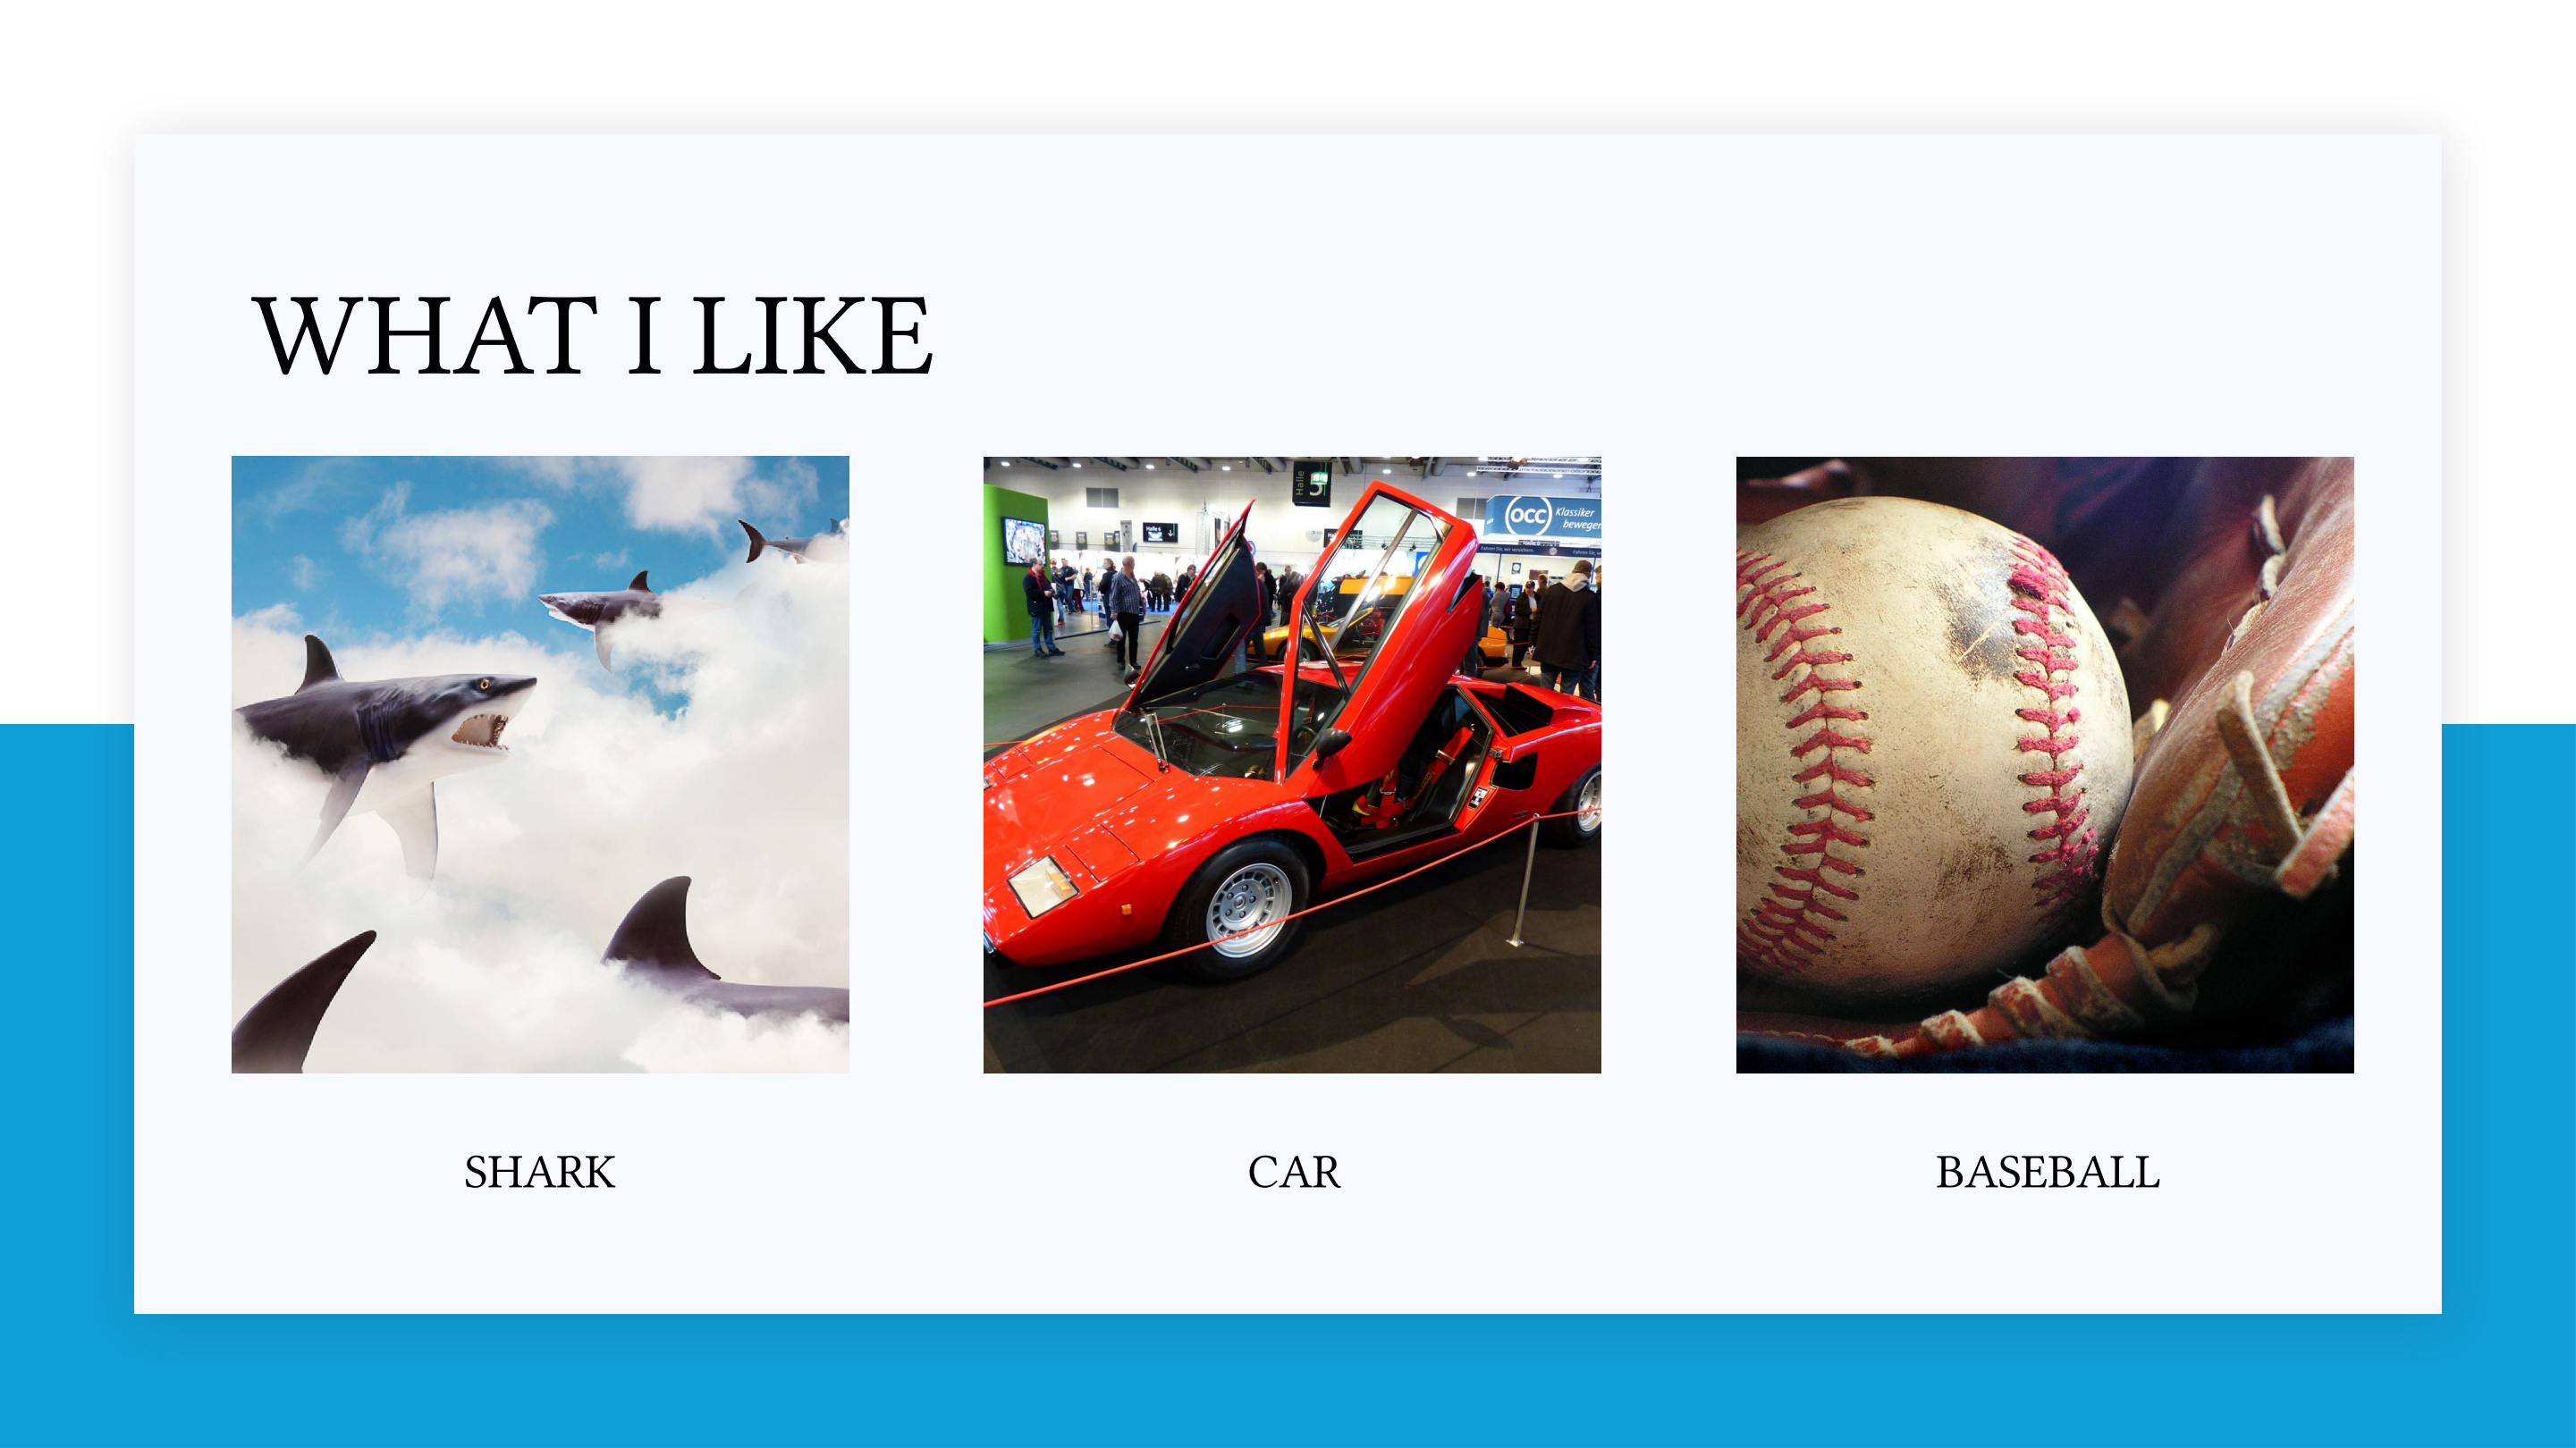
\includegraphics[width=\linewidth]{id31_layout_pass.png}
  {\small （a）通过：三张图片等距分布}
\end{minipage}\hfill
\begin{minipage}[t]{0.485\textwidth}
  \centering
  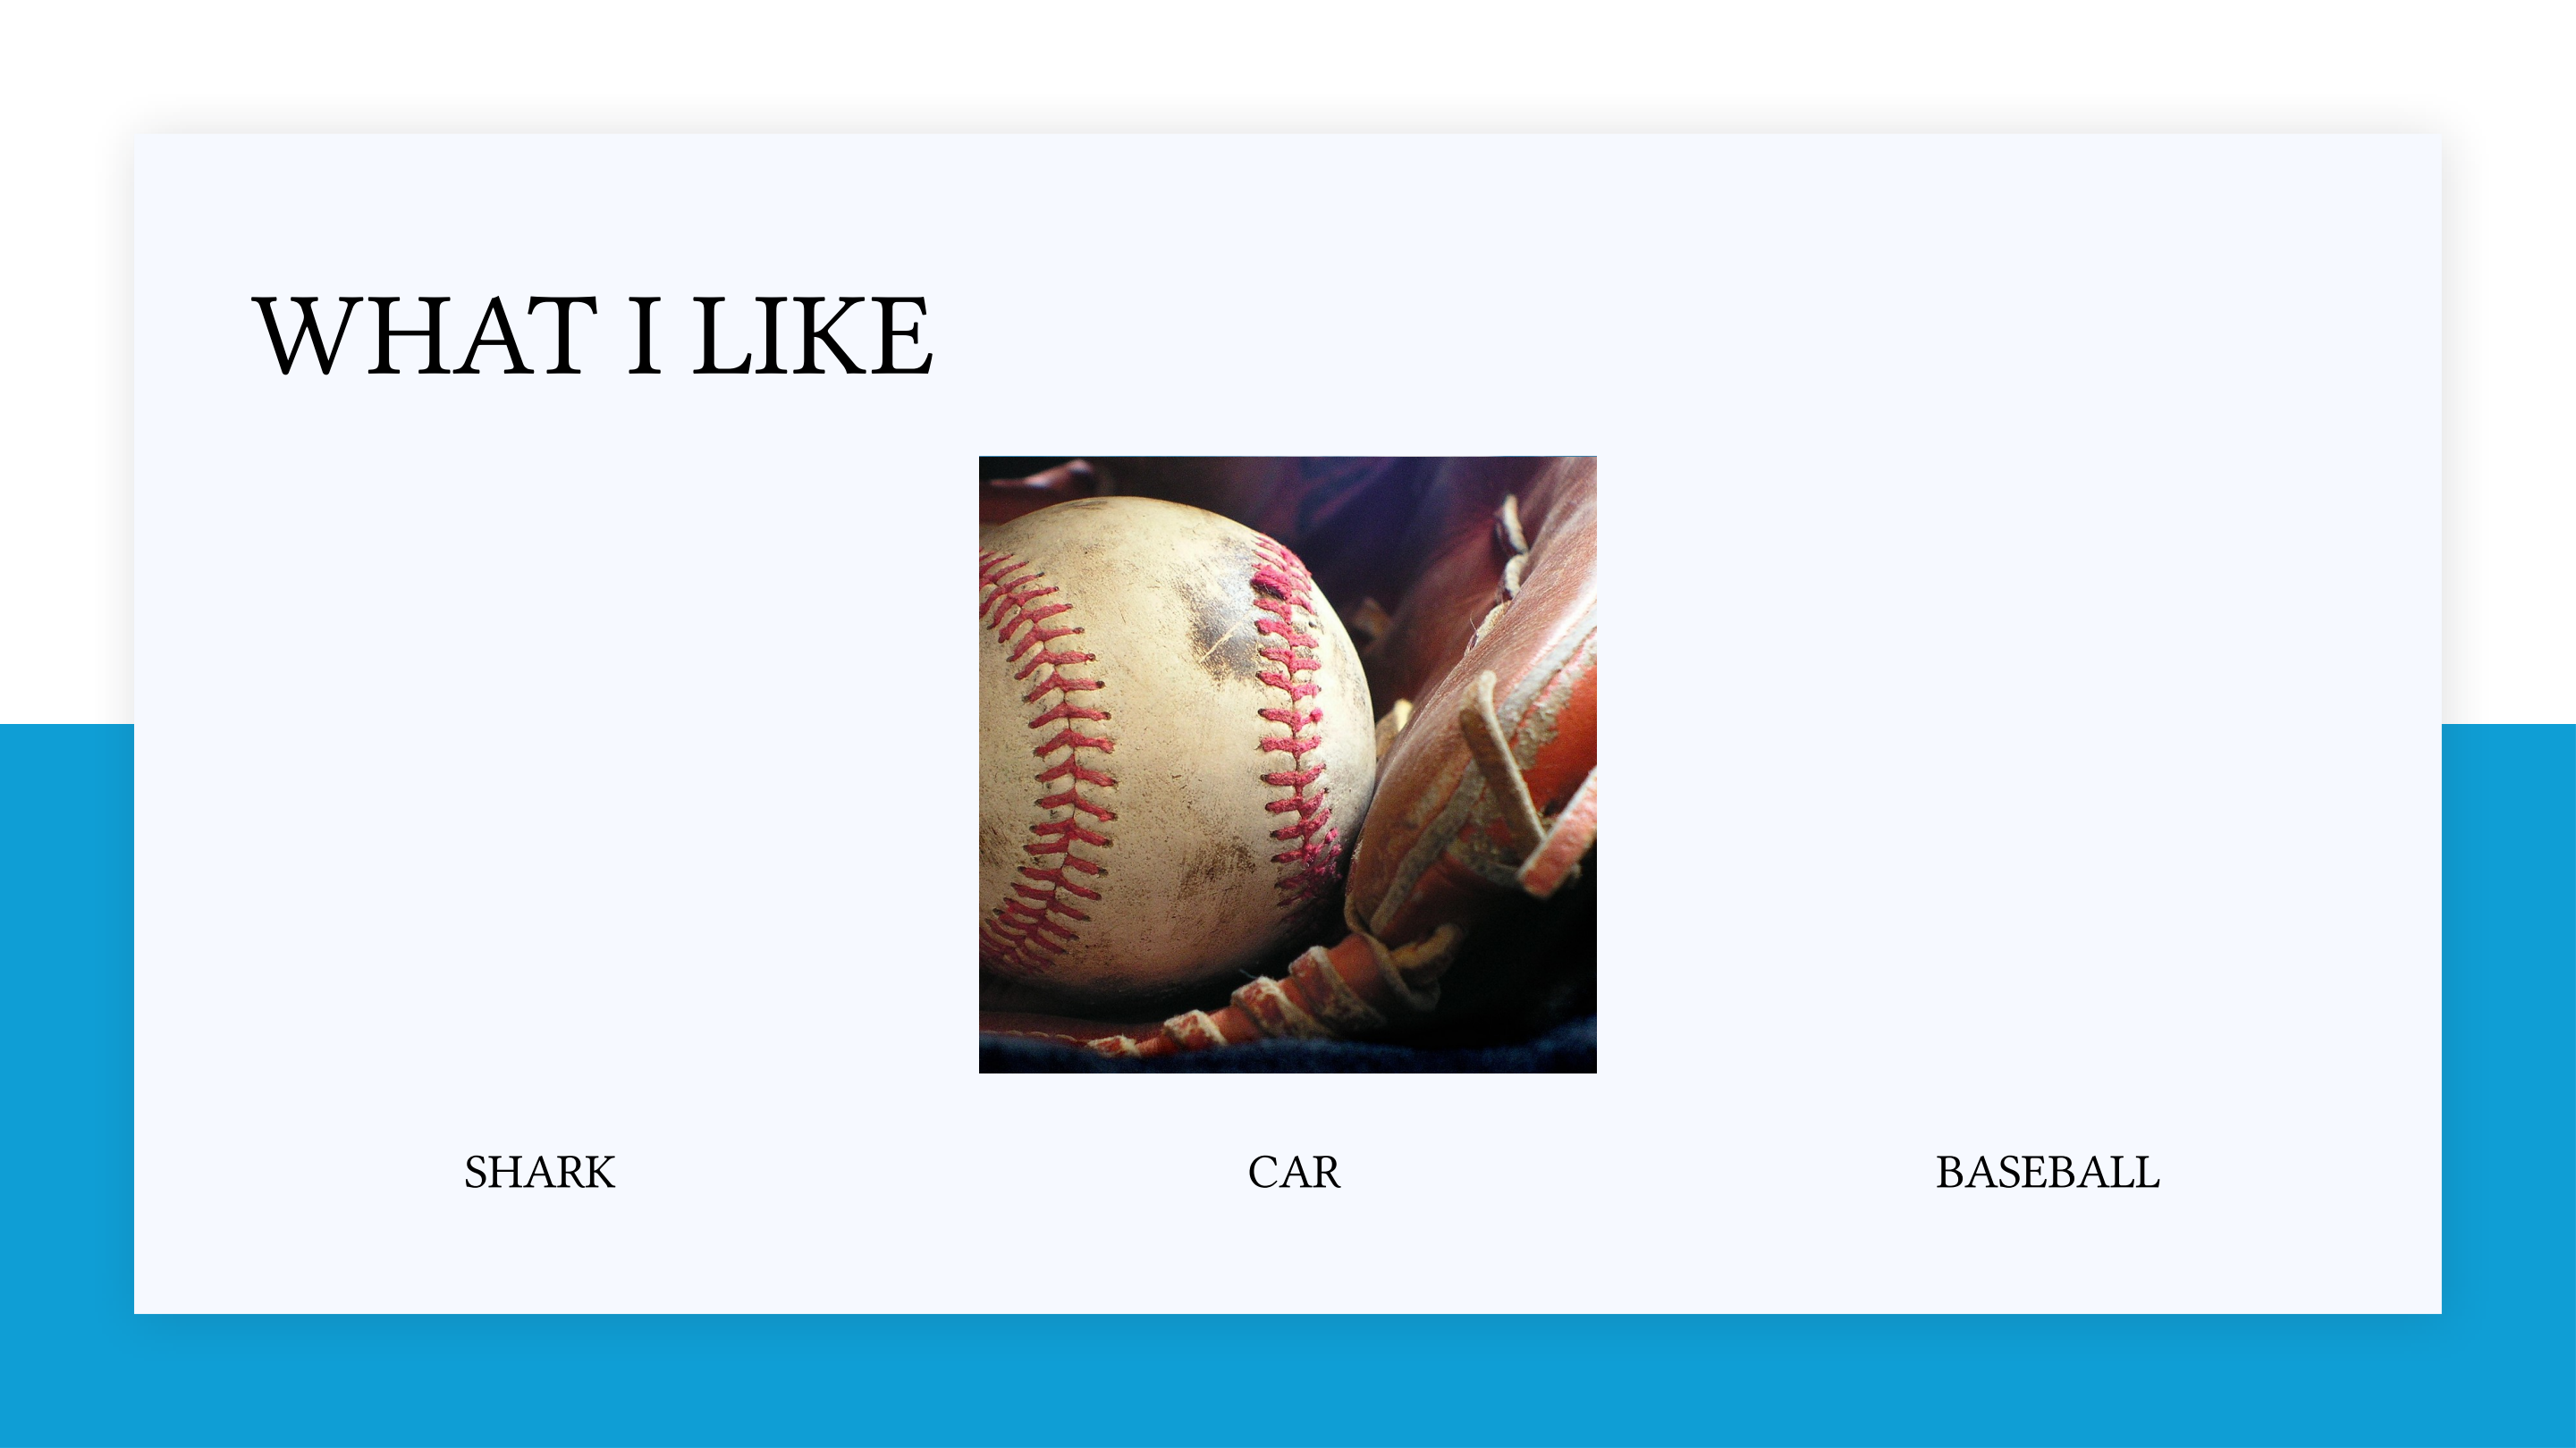
\includegraphics[width=\linewidth]{id31_layout_overlap.png}
  {\small （b）失败：三张图片在中心完全重叠}
\end{minipage}
\caption{id31 实际输出：左图通过；右图三张原图在页面中心重叠，仅显示最上层。}
\end{figure}

ASR-2 与 ASR-6 分别通过 18/32 和 19/32，仅差 3.1 个百分点；一轮与两轮则为 20/32 和 17/32，第二轮下降 9.4 个百分点。四种声学条件的通过数为 9/16、12/16、7/16 和 9/16，未呈稳定趋势。主要瓶颈因此位于 Agent 的空间理解与执行，应由几何验证触发定向重试。

\section{失败、困难与改进}

\subsection{主要失败发生在哪一层}

\begin{table}[H]
\centering
\caption{主要失败环节及证据}
\small
\begin{tabularx}{\textwidth}{L{2.7cm} L{5.4cm} Y}
\toprule
失败环节 & 实验证据 & 主要机制 \\
\midrule
ASR 关键信息丢失 & id20 中，“32 pt”完整保留数由 3/16 提高到 7/16，下游正确数由 2/16 提高到 7/16 & 数值或单位转写错误直接改变编辑参数 \\
Agent 对象与布局规划 & id31 的 57 个现存 PPTX 均保留三张图片，但 17 条发生重叠、3 条发生错位 & 将“整体水平居中排列”误解为“每张图片分别居中”，缺少全局布局约束 \\
生成代码与 API 调用 & 首轮 64 条中 6 条因生成脚本报错触发重试 & 空段落访问 \texttt{runs[0]}、颜色 API、媒体枚举、私有占位符属性和 slide 尺寸属性使用错误 \\
循环控制与结果验证 & id31 从一轮 20/32 降至两轮 17/32；重叠数增加 & 第二轮完整重规划可能覆盖首轮正确结果，系统缺少失败触发、回滚和状态比较 \\
\bottomrule
\end{tabularx}
\end{table}

这些失败不能统一归因于 ASR。以 id20 为例，ASR-2 有一条转写已经保留“32 pt”，但下游仍未完成编辑，说明 Agent 仍可能选错对象或生成错误代码。相反，id31 在两种 ASR 下的首轮通过数均为 10/16，且两种 ASR 在两轮合计中只相差 3.1 个百分点，说明该任务的主要瓶颈位于对象定位和空间规划。

更强的规划或代码模型可能减少语法错误、API 幻觉和部分对象判断错误，但模型能力只是其中一环。如果系统仍依赖自由生成的底层 API 代码，缺少对象清单、类型约束、结果验证和回滚，重叠、错位及破坏已有格式等结构性错误仍可能出现。后续可在固定 ASR、任务和验证器的条件下增加 Agent 模型对照，分别衡量模型能力和工具约束的作用。

\subsection{工程困难及本项目的处理}

\begin{table}[H]
\centering
\caption{工程困难、当前处理与剩余问题}
\small
\begin{tabularx}{\textwidth}{L{3.0cm} Y Y}
\toprule
困难 & 本项目的处理 & 尚未完全解决 \\
\midrule
作者环境耦合 & 改为相对路径，统一输入、输出和模型配置 & 尚缺完整环境锁定与一键部署 \\
GUI 难以批量运行 & 重构 CLI，增加单任务、目录批量和转写复用入口 & 大规模断点恢复和配置清单仍可完善 \\
模型成本与可用性 & 更换为可承受的 DeepSeek 规划与编辑模型 & 尚未形成模型能力、成本和延迟的系统曲线 \\
ASR 与 Agent 错误混合 & 保存转写、日志和输出，并检查关键槽位 & 尚缺完整的槽位级指标和结构化意图层 \\
评价口径不一致 & 为文本、字号、页码建立规则，为布局增加几何与渲染核验 & 仍需统一覆盖更多任务的验证器与人工抽查 \\
\bottomrule
\end{tabularx}
\end{table}

\subsection{后续改进方向}

\begin{enumerate}
  \item 在 ASR 与 Agent 之间加入结构化意图层，显式保存动作、目标对象、属性、数值、单位及指代关系，并在执行前校验关键槽位；
  \item 用类型化编辑工具和对象清单替代自由生成底层 API 代码，限制可调用函数、参数范围和对象作用域；
  \item 建立“规划--执行--验证”闭环，以规则、几何差值和渲染结果触发定向重试，并保留首轮正确结果和回滚点；
  \item 扩展到更多 TSBench 任务、ASR 和 Agent，对照 clean text 上限，统一失败分类并进行置信区间和显著性分析。
\end{enumerate}

\section{研究初衷回看与阶段结论}

\subsection{研究初衷与本阶段定位}

项目最初关注大语言模型如何从语音指令中理解并执行幻灯片编辑。口语中的犹豫、停顿、自我修正和非正式表达，以及带限、噪声和混响等声学变化，都可能使动作、目标对象、属性或数值在转写中损失。因此，原始设想不仅包括将语音转成普通文本，还包括将编辑意图结构化，并比较语音输入与仅使用转写文本时的下游差异。

本报告完成了其中的转写级联系统验证：两种 ASR 处理同一批语音，再由 PPTPilot 执行编辑，并保存转写、日志、PPTX 和核验结果。当前数据还不足以单独估计某一声学条件的稳定效应，但已经可以区分“转写丢失关键信息”和“转写可用但 Agent 执行失败”两类问题。

\subsection{本阶段能够支持的结论}

\begin{itemize}
  \item 转写质量会影响编辑结果，但影响集中在任务关键槽位。Qwen3-ASR 更完整地保留“32 pt”后，id20 正确数由 2/16 提高到 7/16；
  \item 高可读输出率不等于高任务完成率。ASR-6 有 98.44\% 的首轮可读输出，但综合任务核验正确率为 75.00\%；
  \item 正确转写不是任务成功的充分条件。即使关键信息已保留，Agent 仍会因对象选择、空间规划或代码执行失败；
  \item 渲染核验不可缺少。id31 的失败 PPTX 仍包含三张图片，只有查看几何关系和页面渲染才能发现完全遮挡；
  \item 固定增加编辑轮次不能保证改进，验证器触发的定向重试比无条件循环更合理。
\end{itemize}

\subsection{结论边界}

当前实验只覆盖四类任务、两种 ASR 和一个 PPT 编辑 Agent，尚未包含 clean text 上限、结构化意图、speech-native 模型及完整统计检验。因此，结果不能代表完整 Speech2SlideEdit / TSBench 基准，不能证明某种声学条件具有稳定单调影响，也不能据此宣称某个模型具有统计显著优势。其价值在于形成了可复现的系统链路、可追踪的失败证据和后续完整实验所需的评价框架。

\section{结论}

本项目从 PPTArena 论文提出的 PPTPilot 出发，完成了本地化修复、GUI 复现、CLI 重构、双 ASR 接入和语音编辑实验。最终系统能够保存音频转写、Agent 运行过程、编辑后 PPTX 及规则、几何和渲染核验结果，形成了从输入到失败分析的完整证据链。

结果呈现出清楚的层次。流程层面，两种 ASR 的首轮可读输出分别为 61/64 和 63/64；语义层面，更强 ASR 通过保留关键数值与单位，将三项规则任务的正确率从 66.67\% 提高到 79.17\%；执行层面，id31 在两种 ASR 下首轮均只有 10/16 通过，两轮合计通过率为 57.8\%，且第二轮总体低于第一轮。由此可见，ASR 改进能够减少上游信息损失，但 Agent 的对象理解、代码可靠性和结果控制仍是端到端系统的主要限制。

在 id20 / ASR-2 与 id31 / 双 ASR 组成的 48 条匹配样本中，二轮最终正确数由 22/48 降至 20/48，且日志中自动重试触发次数由 3 增至 15。其根本问题是第二轮会同时修复失败与覆盖正确结果，因而不应作为默认策略。

因此，后续工作需同时建设任务关键信息表示、受约束的编辑工具、渲染与几何验证器，以及可回滚的定向重试机制。

\section*{参考资料}

\begin{enumerate}[label={[\arabic*]},leftmargin=2.5em]
  \item Michael Ofengenden, Yunze Man, Ziqi Pang, Yu-Xiong Wang. \textit{PPTArena: A Benchmark for Agentic PowerPoint Editing}. arXiv:2512.03042v2, 2025.
  \item Kyudan Jung et al. \textit{Talk to Your Slides: High-Efficiency Slide Editing via Language-Driven Structured Data Manipulation}. arXiv:2505.11604v4, 2026.
  \item SURF-2026-0425 项目说明与内部实验材料。
  \item 本项目代码、阶段报告、实验输出与审计记录，2026 年 6 月至 7 月。
\end{enumerate}

\appendix
\section{主要产物索引}

\begin{longtable}{L{3.2cm} L{3.3cm} L{8.0cm}}
\toprule
产物 & 角色 & 内容 \\
\midrule
\endfirsthead
\toprule
产物 & 角色 & 内容 \\
\midrule
\endhead
PPTArena-main & 原始基线 & 论文代码与本地修复起点 \\
PPTArena\_GUI & GUI 复现 & 本地预览、模型选择、错误处理和结果保存 \\
PPTArena\_CLI & 批量底座 & 单任务与批量入口，去除 Web 依赖 \\
GUI / CLI 早期结果对比 & 探索性实验 & 从 PPTArena 数据集选取的 10 个案例及其输入、输出和 GUI / CLI 记录；不构成严格配对比较 \\
PPTAgent & 第一版语音扩展 & 双 ASR、任务映射和转写保存 \\
Agent & 最终实验版 & 统一入口、DeepSeek、四任务输出、规则与几何核验、逐样本审计及最终报告 \\
SSFT260706\_1 / \_2 & 音频合集 & 四种口语变体及 clean、bandlimit、noise、reverb 声学条件 \\
\bottomrule
\end{longtable}

\end{document}
